% Capítulo 12: C++ compila para um sistema; Java compila para bytecode, que roda em qualquer JVM.
\documentclass[border=4pt]{standalone}
\usepackage[utf8]{inputenc}
\usepackage[T1]{fontenc}
% Estilo comum dos fluxogramas e diagramas de blocos.
\usepackage{tikz}
\usetikzlibrary{arrows.meta, positioning, calc, shapes.geometric, shapes.misc}
\definecolor{navy}{RGB}{23,45,80}
\definecolor{laranja}{RGB}{250,110,29}
\definecolor{cinzalogo}{RGB}{107,114,126}
\definecolor{azul}{RGB}{205,222,247}
\tikzset{
  base/.style={draw=navy, line width=0.9pt, font=\sffamily\small, align=center, inner sep=4pt},
  terminal/.style={base, rounded rectangle, fill=laranja!45, draw=laranja, minimum width=20mm, minimum height=7mm},
  processo/.style={base, rectangle, fill=laranja!12, minimum width=28mm, minimum height=8mm},
  decisao/.style={base, diamond, aspect=2.2, fill=azul, inner sep=1pt, minimum width=30mm},
  es/.style={base, trapezium, trapezium left angle=72, trapezium right angle=108,
             fill=white, minimum width=26mm, minimum height=8mm, trapezium stretches body},
  fluxo/.style={-{Stealth[length=2.2mm]}, navy, line width=0.9pt},
  rotulo/.style={font=\sffamily\small\bfseries, text=navy},
  legenda/.style={font=\sffamily\scriptsize, text=cinzalogo},
  resposta/.style={font=\sffamily\scriptsize\bfseries, text=navy},
}

\tikzset{
  arq/.style={base, rectangle, rounded corners=2pt, fill=white, font=\ttfamily\small, minimum width=20mm, minimum height=8mm},
  ferr/.style={base, rectangle, fill=laranja!25, minimum width=18mm, minimum height=8mm, font=\ttfamily\small},
  so/.style={base, rectangle, rounded corners=2pt, fill=azul, minimum width=26mm, minimum height=7mm, font=\sffamily\scriptsize},
  sonao/.style={so, fill=white, draw=cinzalogo!60, dashed, text=cinzalogo},
}
\begin{document}
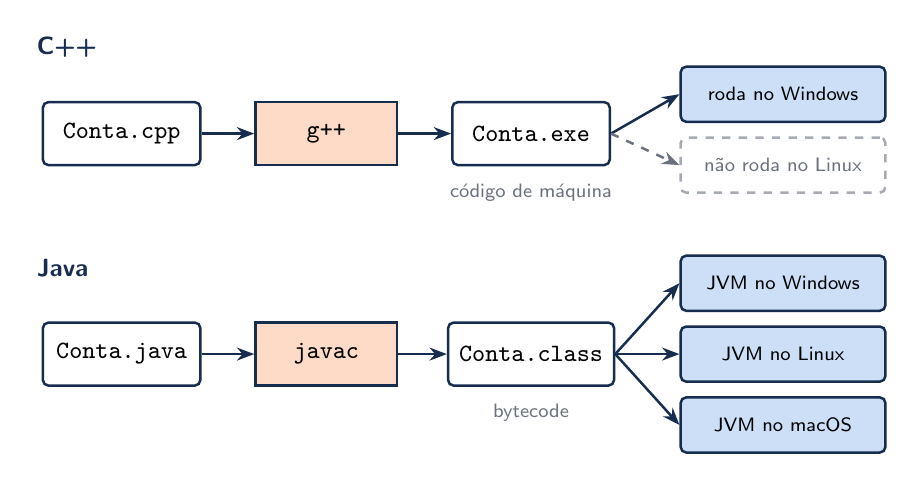
\begin{tikzpicture}
  % C++
  \node[rotulo, anchor=west] at (-1.2, 1.1) {C++};
  \node[arq] (cpp) at (0, 0) {Conta.cpp};
  \node[ferr] (gpp) at (2.6, 0) {g++};
  \node[arq] (exe) at (5.2, 0) {Conta.exe};
  \node[so] (w1) at (8.4, 0.5) {roda no Windows};
  \node[sonao] (l1) at (8.4, -0.4) {não roda no Linux};
  \draw[fluxo] (cpp) -- (gpp);
  \draw[fluxo] (gpp) -- (exe);
  \draw[fluxo] (exe.east) -- (w1.west);
  \draw[fluxo, cinzalogo, dashed] (exe.east) -- (l1.west);
  \node[legenda] at (5.2, -0.75) {código de máquina};

  % Java
  \node[rotulo, anchor=west] at (-1.2, -1.7) {Java};
  \node[arq] (java) at (0, -2.8) {Conta.java};
  \node[ferr] (javac) at (2.6, -2.8) {javac};
  \node[arq] (class) at (5.2, -2.8) {Conta.class};
  \node[so] (w2) at (8.4, -1.9) {JVM no Windows};
  \node[so] (l2) at (8.4, -2.8) {JVM no Linux};
  \node[so] (m2) at (8.4, -3.7) {JVM no macOS};
  \draw[fluxo] (java) -- (javac);
  \draw[fluxo] (javac) -- (class);
  \foreach \d in {w2, l2, m2} { \draw[fluxo] (class.east) -- (\d.west); }
  \node[legenda] at (5.2, -3.55) {bytecode};
\end{tikzpicture}
\end{document}
